\documentclass[12pt,letterpaper]{report}

% Packages and shared commands. Keep chapter files focused on content.
\usepackage{amsmath,amssymb,amsthm}
\usepackage{physics} % \dd is the differential operator.
\usepackage{natbib}
\usepackage{graphicx}
\graphicspath{{Rnw/}} % Resolve figures generated in the Rnw folder.
% Place floats after their source, never before introduction.
\usepackage{flafter}
\usepackage[section]{placeins} % Keep floats within their explanatory section.
\usepackage{booktabs}
\usepackage{url}
\usepackage{alltt,xcolor}
\usepackage{etoolbox}
\usepackage{algorithm}
\usepackage{algpseudocode}
\usepackage{uconnthesis}
% Subtle dark-blue text makes clickable references and URLs visible.
\definecolor{thesislink}{RGB}{35,65,105}
\usepackage[pdfusetitle,colorlinks=true,
  linkcolor=thesislink,citecolor=thesislink,urlcolor=thesislink]{hyperref}
\AtBeginDocument{\hypersetup{pdfauthor={\thesisauthor}}}

% Let floats share text pages more freely instead of being deferred.
% Fractions refer to the text area's height: allow up to 85% at the top
% or 65% at the bottom, with at least 10% reserved for text.
\renewcommand{\topfraction}{0.85}
\renewcommand{\bottomfraction}{0.65}
\renewcommand{\textfraction}{0.10}
\setcounter{topnumber}{3}
\setcounter{bottomnumber}{3}
\setcounter{totalnumber}{5}

% Normally create a float-only page only when floats fill at least 80%.
% Keep this threshold below topfraction so medium-sized floats can still
% fit at the top of a text page. A chapter end, \clearpage, or the section
% barriers from placeins can still flush floats onto their own pages.
% These settings reduce isolated floats; they do not prohibit float pages.
\renewcommand{\floatpagefraction}{0.80}
% Corresponding settings for full-width floats in a two-column document.
\renewcommand{\dbltopfraction}{0.85}
\renewcommand{\dblfloatpagefraction}{0.80}
\setcounter{dbltopnumber}{3}

\newcommand{\RR}{\mathbb{R}}

\setlength{\unitlength}{1mm}
% Default LaTeX setup generated by knitr; keep it outside the appendix.
\definecolor{fgcolor}{rgb}{0.345, 0.345, 0.345}
\newcommand{\hlnum}[1]{\textcolor[rgb]{0.686,0.059,0.569}{#1}}%
\newcommand{\hlsng}[1]{\textcolor[rgb]{0.192,0.494,0.8}{#1}}%
\newcommand{\hlcom}[1]{\textcolor[rgb]{0.678,0.584,0.686}{\textit{#1}}}%
\newcommand{\hlopt}[1]{\textcolor[rgb]{0,0,0}{#1}}%
\newcommand{\hldef}[1]{\textcolor[rgb]{0.345,0.345,0.345}{#1}}%
\newcommand{\hlkwa}[1]{\textcolor[rgb]{0.161,0.373,0.58}{\textbf{#1}}}%
\newcommand{\hlkwb}[1]{\textcolor[rgb]{0.69,0.353,0.396}{#1}}%
\newcommand{\hlkwc}[1]{\textcolor[rgb]{0.333,0.667,0.333}{#1}}%
\newcommand{\hlkwd}[1]{\textcolor[rgb]{0.737,0.353,0.396}{\textbf{#1}}}%
\let\hlipl\hlkwb

\usepackage{framed}
\makeatletter
\newenvironment{kframe}{%
 \def\at@end@of@kframe{}%
 \ifinner\ifhmode%
  \def\at@end@of@kframe{\end{minipage}}%
  \begin{minipage}{\columnwidth}%
 \fi\fi%
 \def\FrameCommand##1{\hskip\@totalleftmargin \hskip-\fboxsep
 \colorbox{shadecolor}{##1}\hskip-\fboxsep
     % There is no \\@totalrightmargin, so:
     \hskip-\linewidth \hskip-\@totalleftmargin \hskip\columnwidth}%
 \MakeFramed {\advance\hsize-\width
   \@totalleftmargin\z@ \linewidth\hsize
   \@setminipage}}%
 {\par\unskip\endMakeFramed%
 \at@end@of@kframe}
\makeatother

\definecolor{shadecolor}{rgb}{.97, .97, .97}
\definecolor{messagecolor}{rgb}{0, 0, 0}
\definecolor{warningcolor}{rgb}{1, 0, 1}
\definecolor{errorcolor}{rgb}{1, 0, 0}
\newenvironment{knitrout}{}{} % an empty environment to be redefined in TeX


\AtBeginEnvironment{knitrout}{\singlespacing}


% To review selected chapters, uncomment ONE of the examples below.
% \includeonly skips other \include files; keep the \include commands below.
% Front matter and files loaded with \input are still included.
% This produces a partial draft, not a complete dissertation.
% \includeonly{chap1}       % Chapter 1 only; skip Chapters 2, 3, and appendices.
% \includeonly{chap1,chap3} % Chapters 1 and 3; skip Chapter 2 and appendices.
% Comment out \includeonly again to build the complete dissertation.

\title{A Sample Dissertation in Statistics}
\name{Student Full Name}
\myPreviousDegreeLong{B.S., University Name, 2020 \\ M.S., University Name, 2022}
\myPreviousDegreeShort{B.S., M.S.}
\degree{Doctor of Philosophy}
\myNewDegreeShort{Ph.D.}
\dept{Statistics}
\thesistype{Dissertation}
% Set the graduation year explicitly so future builds retain the same date.
\copyrightyear{2026}
\myMajorAdvisor{Advisor Full Name}
% For two co-major advisors, comment out \myMajorAdvisor above and use both:
% \myCoAdvisorA{First Co-Major Advisor Full Name}
% \myCoAdvisorB{Second Co-Major Advisor Full Name}
\myAssociateAdvisorA{Committee Member One}
\myAssociateAdvisorB{Committee Member Two}
% \myAssociateAdvisorC{Committee Member Three}
% \myAssociateAdvisorD{Committee Member Four}

% Optional front matter; comment out any unwanted page or list.
\copyrighttrue
\figurespagetrue
\tablespagetrue
\signaturelinestrue % Signature spaces for a printed committee copy.
% Comment out \signaturelinestrue for an approval page with names only.

\begin{document}

% Dissertation abstract: required, unnumbered, and before the title page.
\firstpage
This sample dissertation demonstrates the structure of a University of
Connecticut statistics dissertation. Replace this paragraph with a summary
of the research question, methods, principal findings, and conclusions.
The dissertation abstract must not exceed 350 words in total.


The abstract need not be a single paragraph. Prefer multiple paragraphs to
separate the research question, methods, findings, and conclusions when that
structure improves readability. The 350-word limit applies to the entire
abstract, not to each paragraph. With this template's double spacing and
heading layout, an abstract within that limit may occupy up to two pages.


\beforepreface
\prefacesection{Dedication}
To the people who encouraged this work.

\prefacesection{Acknowledgments}
Thank the people and organizations that supported your research here.
Include funding acknowledgments required by your sponsors.

\afterpreface

% Basic LaTeX examples adapted from Leslie Lamport.
\chapter{Introduction}
\label{introduction}


This template demonstrates how to present mathematical statements, equations,
lists, tables, figures, algorithms, code, output, and references in a thesis.
For writing conventions, follow \citet{schifano2026statistical}, available at
\url{https://statds.github.io/stat-writing/}. The University of Connecticut's
requirements govern thesis formatting.


\section{Basic LaTeX examples}
These source examples illustrate conventions described by
\citet{lamport1994latex}.


\subsection{Ordinary text}


The ends of words and sentences are marked by spaces. It doesn't matter how
many spaces you type; one is as good as 100. The end of a line counts as a
space.\footnote{ This is a sample input file. Comparing it with the output it
generates can show you how to produce a simple document of your own. }


One or more blank lines denote the end of a paragraph.


Since any number of consecutive spaces are treated like a single one, the
formatting of the input file makes no difference to \LaTeX, but it makes a
difference to you. When you use \LaTeX, making your input file as easy to read
as possible will be a great help as you write your document and when you change
it. Keep explanatory comments brief and separate them from the thesis text.


Because printing is different from typewriting, there are a number of things
that you have to do differently when preparing an input file than if you were
just typing the document directly. Quotation marks like ``this'' have to be
handled specially, as do quotes within quotes: ``\,`this' is what I just wrote,
not `that'\,.''


Dashes come in three sizes: an intra-word dash, a medium dash for number ranges
like 1--2, and a punctuation dash---like this.


A sentence-ending space should be larger than the space between words within a
sentence. You sometimes have to type special commands in conjunction with
punctuation characters to get this right, as in the following sentence. Gnats,
gnus, etc.\ all begin with G\@. You should check the spaces after periods when
reading your output to make sure you haven't forgotten any special cases.
Generating an ellipsis \ldots\ with the right spacing around the periods
requires a special command.


\LaTeX\ interprets some common characters as commands, so you must type special
commands to generate them. These characters include the following: \$ \& \% \#
\{ and \}.


In printing, text is emphasized by using an {\em italic\/} type style.


\begin{em}
  A long segment of text can also be emphasized in this way. Text within such a
  segment given additional emphasis with\/ {\em Roman} type. Italic type loses
  its ability to emphasize and become simply distracting when used excessively.
\end{em}


It is sometimes necessary to prevent \LaTeX\ from breaking a line where it
might otherwise do so. This may be at a space, as between the ``Mr.'' and
``Jones'' in ``Mr.~Jones,'' or within a word---especially when the word is a
symbol like \mbox{\em itemnum\/} that makes little sense when hyphenated across
lines.


Footnotes\footnote{This is an example of a footnote.} pose no problem.


\LaTeX\ is good at typesetting mathematical formulas like
$\widehat{\mu}=\bar{x}$ or
\[
  \operatorname{SE}(\overline{X}) = \sigma/\sqrt{n}.
\]


Remember that a letter like $x$ is a formula when it denotes a mathematical
symbol, and should be treated as one.


\subsection{Displayed text}


Text is displayed by indenting it from the left margin.


\subsubsection{Quotations}


Quotations are commonly displayed. There are short quotations
\begin{quote}
  This is a short quotation. It consists of a single paragraph of text. There
  is no paragraph indentation.
\end{quote}
and longer ones.
\begin{quotation}
  This is a longer quotation. It consists of two paragraphs of text. The
  beginning of each paragraph is indicated by an extra indentation.


  This is the second paragraph of the quotation. It is just as dull as the
  first paragraph.
\end{quotation}


\subsubsection{Lists}


Another frequently-displayed structure is a list.


\paragraph{Itemize.}
The following is an example of an {\em itemized} list.


\begin{quote}
  \begin{itemize}
    \item  This is the first item of an itemized list.  Each item
    in the list is marked with a ``tick''. The document style determines what
    kind of tick mark is used.


    \item  This is the second item of the list.  It contains another
    list nested inside it. The inner list is an {\em enumerated} list.
    \begin{enumerate}
      \item This is the first item of an enumerated list that
      is nested within the itemized list.


      \item This is the second item of the inner list.  \LaTeX\
      allows you to nest lists deeper than you really should.
    \end{enumerate}
    This is the rest of the second item of the outer list. It is no more
    interesting than any other part of the item.
    \item  This is the third item of the list.
  \end{itemize}
\end{quote}


\paragraph{Verse.}
You can even display poetry.


\begin{quote}
  \begin{quote}
    \begin{verse}
      There is an environment for verse \\
      Whose features some poets will curse.


      For instead of making\\
      Them do {\em all\/} line breaking, \\
      It allows them to put too many words on a line when they'd
      rather be forced to be terse.
    \end{verse}
  \end{quote}
\end{quote}


\subsubsection{Mathematics}
Displayed formulas may occupy one or several lines. Use the environments
provided by \texttt{amsmath} for multiline equations.
\[
  Y_i = \beta_0+\beta_1 x_i+\varepsilon_i.
\]
Don't start a paragraph with a displayed equation, nor make one a paragraph by
itself.


\section{Sampling and estimation}
Suppose a study records independent observations $X_1,\ldots,X_n$ from a
population with mean $\mu$ and variance $\sigma^2$, where $n\geq 1$ and
$0<\sigma^2<\infty$. The estimand is the population mean. An estimator is a
rule applied to the random sample; an estimate is its value for the observed
data. This distinction separates uncertainty before sampling from a number
reported after analysis \citep{wasserman2004all}.


\begin{definition}[Bias]
  The bias of an estimator $T$ of $\mu$, when its expectation exists, is
  \[
    \operatorname{Bias}_{\mu}(T) = \mathbb{E}_{\mu}(T)-\mu.
  \]
  An estimator is unbiased when its bias is zero for every population in the
  specified model.
\end{definition}
The sample mean is the estimator
\begin{equation}
  \label{eq:random-sample-mean}
  \overline{X} = \frac{1}{n}\sum_{i=1}^{n}X_i.
\end{equation}
Equation~\eqref{eq:random-sample-mean} uses uppercase letters for random
variables. Lowercase $x_i$ and $\bar{x}$ denote their observed values.


\begin{theorem}[Properties of the sample mean]
  \label{thm:sample-mean-properties}
  Under the stated sampling assumptions, $\overline{X}$ is unbiased for $\mu$
  and has variance $\sigma^2/n$.
\end{theorem}
\begin{proof}
  Linearity of expectation gives
  \[
    \mathbb{E}(\overline{X})
    = \frac{1}{n}\sum_{i=1}^{n}\mathbb{E}(X_i) = \mu.
  \]
  Independence makes the pairwise covariances zero, so
  \[
    \operatorname{Var}(\overline{X})
    = \frac{1}{n^2}\sum_{i=1}^{n}\operatorname{Var}(X_i)
    = \frac{\sigma^2}{n}.
  \]
\end{proof}
\begin{corollary}[Precision and sample size]
  Under the assumptions of Theorem~\ref{thm:sample-mean-properties}, the
  standard error of $\overline{X}$ is $\sigma/\sqrt{n}$. Multiplying the
  sample size by four halves this standard error.
\end{corollary}
\begin{proof}
  Take the square root of the variance and replace $n$ by $4n$.
\end{proof}
The standard error describes variation across samples. It differs from the
population standard deviation, which describes variation among individuals.
When $\sigma$ is unknown, estimate it rather than reporting the formula as
though the population variance were known.


\section{Assumptions and interpretation}
Unbiasedness alone does not establish that an estimator is useful. Report its
variability, the assumptions behind its uncertainty calculation, and the
population to which the conclusions apply. Independence deserves particular
attention when observations come from repeated measurements or clusters.
Chapter~\ref{chap:normal-mean} develops a confidence interval under an explicit
normal sampling model.


\begin{remark}
  Increasing sample size reduces sampling variability under this model. It
  does not automatically remove selection bias, measurement error, or model
  misspecification.
\end{remark}

\chapter{Estimating a Normal Population Mean}
\label{chap:normal-mean}


This worked example shows how to connect a statistical model, an estimator,
an uncertainty statement, and an interpretation. The observations are
illustrative; they do not represent a scientific study. General treatments of
estimation and confidence intervals are given by \citet{wasserman2004all}.


\section{Model and estimand}
Assume $X_1,\ldots,X_n$ are independent normal random variables with mean
$\mu$ and variance $\sigma^2$, where $n\geq 2$ and $\sigma^2>0$. The target is
$\mu$, the population mean. For observed values $x_1,\ldots,x_n$, the density
of one observation is
\begin{equation}
  \label{eq:normal-density}
  f(x;\mu,\sigma^2)
  = \frac{1}{\sqrt{2\pi\sigma^2}}
    \exp\left\{-\frac{(x-\mu)^2}{2\sigma^2}\right\},
  \qquad x\in\RR.
\end{equation}
Equation~\eqref{eq:normal-density} specifies the sampling model, not a
probability distribution on the unknown parameter $\mu$.


\section{Maximum likelihood estimation}
The log likelihood is
\begin{equation}
  \label{eq:normal-loglikelihood}
  \ell(\mu,\sigma^2)
  = -\frac{n}{2}\log(2\pi\sigma^2)
    -\frac{1}{2\sigma^2}\sum_{i=1}^{n}(x_i-\mu)^2.
\end{equation}
Holding $\sigma^2$ fixed in Equation~\eqref{eq:normal-loglikelihood},
differentiation with respect to $\mu$ gives
\begin{align*}
  \frac{\partial\ell}{\partial\mu}
    &= \frac{1}{\sigma^2}\sum_{i=1}^{n}(x_i-\mu), \\
  \frac{\partial^2\ell}{\partial\mu^2}
    &= -\frac{n}{\sigma^2}<0.
\end{align*}
The score is zero at $\widehat{\mu}=\bar{x}$. The negative second derivative
shows that this is the unique maximizer in $\mu$ for each fixed variance.
If the observed values are not all equal, joint maximization also gives
$\widehat{\sigma}^2_{\mathrm{ML}}
= n^{-1}\sum_{i=1}^{n}(x_i-\bar{x})^2$. This variance estimate differs from
the unbiased sample variance used below. For identical observations, the
joint likelihood has no finite maximizer with $\sigma^2>0$.


\section{Confidence intervals}
\begin{prop}[Normal-mean pivot]
  \label{prop:normal-pivot}
  Under the normal sampling model, define
  \[
    S^2 = \frac{1}{n-1}\sum_{i=1}^{n}(X_i-\overline{X})^2.
  \]
  Then
  \begin{equation}
    \label{eq:normal-pivot}
    T = \frac{\overline{X}-\mu}{S/\sqrt{n}}\sim t_{n-1}.
  \end{equation}
\end{prop}
\begin{proof}
  The standardized mean is standard normal, $(n-1)S^2/\sigma^2$ has a
  chi-squared distribution with $n-1$ degrees of freedom, and these two
  quantities are independent. Their ratio, with the chi-squared quantity
  divided by its degrees of freedom and square-rooted, has the stated
  Student distribution.
\end{proof}
Let $t_{\nu,p}$ denote the $p$ quantile of a Student distribution with $\nu$
degrees of freedom. Proposition~\ref{prop:normal-pivot} and
Equation~\eqref{eq:normal-pivot} give a $100(1-\alpha)\%$ confidence interval
for $\mu$, for $0<\alpha<1$:
\begin{equation}
  \label{eq:mean-confidence-interval}
  \left[\bar{x}-t_{n-1,1-\alpha/2}\frac{s}{\sqrt{n}},\quad
        \bar{x}+t_{n-1,1-\alpha/2}\frac{s}{\sqrt{n}}\right].
\end{equation}
Here $s$ is the observed sample standard deviation. Appendix~\ref{app:variance}
explains the $n-1$ denominator in the sample variance.


For the illustrative values $1,2,3$, we have $n=3$, $\bar{x}=2$, and $s=1$.
Using $t_{2,0.975}\approx 4.303$ in
Equation~\eqref{eq:mean-confidence-interval} gives a 95\% confidence interval
of approximately $[-0.484,4.484]$. The wide interval reflects the uncertainty
associated with three observations. These values demonstrate a calculation;
they do not provide evidence for the normal sampling assumption.


\begin{remark}[Coverage]
  The interval procedure covers the fixed population mean in 95\% of repeated
  samples under the stated model. A realized frequentist interval does not
  assign a 95\% probability to the fixed parameter. Exact coverage relies on
  normality and independence; a small sample alone does not justify a normal
  approximation.
\end{remark}


\section{Planning a simulation study}
A simulation can examine interval coverage when the sampling model changes.
Before generating data, specify the aim, data-generating mechanisms, estimand,
methods, and performance measures \citep{morris2019using}. For example,
compare normal and skewed populations with the same mean and variance, vary
sample size, and evaluate the interval in
Equation~\eqref{eq:mean-confidence-interval}.


Report the repetition count, Monte Carlo uncertainty, and failed fits.
Retain reproducible code. This template reports no simulation results.

\chapter{Statistical Reporting Examples}
\label{chap:presentation}
This chapter illustrates statistical presentation with tables, figures,
algorithms, code, output, and reference formats. Replace the demonstration
content with your research while retaining the patterns you need.


\section{Writing style}
Follow \citet{schifano2026statistical} when preparing the thesis. Their guide,
\emph{Statistical Writing}, is available at
\url{https://statds.github.io/stat-writing/}. Its chapters on writing tools and
manuscript sections provide guidance on source preparation, mathematical
exposition, and statistical reporting. University requirements govern the
document layout and front matter.


Introduce the research problem, explain the gap in existing work, and state the
contribution. Define notation consistently and state assumptions before
presenting theoretical results. The abstract should stand on its own, summarize
the contribution, and avoid citations. Discuss the meaning of results rather
than repeating every value from tables and figures.


Treat equations as parts of sentences and punctuate them accordingly. Before
a displayed equation, ``is'' is sufficient; ``is given by'' is unnecessary. Use
descriptive labels and refer to equations with \verb|\eqref|. Refer to each
table and figure in the text; give each an informative, self-contained caption.
Use present tense for exposition and past tense for completed experiments.
Treat ``data'' as plural and reserve ``significant'' for its statistical
meaning.


\section{Mathematical statements and proofs}
\begin{definition}
  For $n>0$ observations $x_1,\ldots,x_n\in\RR$, the sample mean is
  \begin{equation}
    \label{eq:sample-mean}
    \bar{x} = \frac{1}{n} \sum_{i=1}^{n} x_i.
  \end{equation}
\end{definition}
\begin{theorem}
  \label{thm:constant-mean}
  If every observation equals $c$, then $\bar{x}=c$.
\end{theorem}
\begin{proof}
  Substitution in Equation~\eqref{eq:sample-mean} gives $nc/n=c$.
\end{proof}
\begin{corollary}
  The sample mean of a sequence of zeros is zero.
\end{corollary}
\begin{proof}
  Apply Theorem~\ref{thm:constant-mean} with $c=0$.
\end{proof}
Equation~\eqref{eq:centered-zero} shows that the centered observations sum to
zero. An aligned derivation gives:
\begin{align}
  \sum_{i=1}^{n}(x_i-\bar{x}) &= \sum_{i=1}^{n} x_i - n \bar{x}
  \notag\\
  &= 0.\label{eq:centered-zero}
\end{align}


\section{Differentiation and integration}
A probability density with two cases is
\begin{equation}
  \label{eq:piecewise-density}
  f(x) =
  \begin{cases}
    2x, & 0<x<1, \\
    0, & \text{otherwise}.
  \end{cases}
\end{equation}
The comma after the first condition separates the cases; the period after
``otherwise'' ends the sentence. Keep this punctuation inside the cases
rather than adding another period after the closing brace.


Use \verb|\dd| from the \texttt{physics} package for the upright differential
operator in derivatives and integration measures. For a random variable
with density $f(x)=2x$ on $0<x<1$ and zero elsewhere, normalization gives
\[
  \int_0^1 f(x)\dd{x}=\int_0^1 2x\dd{x}=1.
\]
Its expectation is obtained by integrating $x$ against the density:
\[
  \mathbb{E}(X)=\int_0^1 x f(x)\dd{x}=\frac{2}{3}.
\]
Within the support, the logarithmic derivative is
\[
  \frac{\dd}{\dd x}\log f(x)=\frac{1}{x}.
\]


\section{Lists}
\begin{itemize}
  \item Describe the research question.
  \item Explain the method and assumptions.
  \item Present results and their limitations.
\end{itemize}
\begin{enumerate}
  \item Read the observations.
  \item Calculate their mean.
  \item Check the calculation against a known example.
\end{enumerate}
\begin{description}
  \item[Input] A nonempty sequence of observations.
  \item[Output] Its arithmetic mean.
\end{description}


\section{Tables and figures}
For figure and table style tips, follow the guidance in
\emph{Statistical Writing} \citep{schifano2026statistical}, available at
\url{https://statds.github.io/stat-writing/}. Use that guide when preparing
plots, formatting tables, and writing captions for your thesis.


Table captions conventionally precede the table; figure captions follow the
illustration. Put labels after captions and refer to them by label.
Table~\ref{tab:sample-data} summarizes the values plotted in
Figure~\ref{fig:sample-data}.
\begin{table}[tbp]
  \centering
  \caption{Three observations, $x_1 = 1$, $x_2 = 2$, and $x_3 = 3$,
  and their arithmetic mean.}\label{tab:sample-data}
  \begin{tabular}{lr}
    \toprule
    Quantity & Value \\
    \midrule
    First observation & 1 \\
    Second observation & 2 \\
    Third observation & 3 \\
    Sample mean & 2 \\
    \bottomrule
  \end{tabular}
\end{table}
\begin{figure}[tbp]
  \centering
  \begin{picture}(80,40)
    \put(10,8){\vector(1,0){60}}
    \put(10,8){\vector(0,1){28}}
    \put(70,3){\makebox(0,0){$i$}}
    \put(5,35){\makebox(0,0){$x_i$}}
    \put(25,16){\circle*{2}}
    \put(40,24){\circle*{2}}
    \put(55,32){\circle*{2}}
    \put(9,16){\line(1,0){2}}
    \put(9,24){\line(1,0){2}}
    \put(9,32){\line(1,0){2}}
    \put(6,16){\makebox(0,0){1}}
    \put(6,24){\makebox(0,0){2}}
    \put(6,32){\makebox(0,0){3}}
    \put(25,4){\makebox(0,0){1}}
    \put(40,4){\makebox(0,0){2}}
    \put(55,4){\makebox(0,0){3}}
  \end{picture}
  \caption{Observation values $x_i = i$ for indices $i = 1, 2, 3$.
  The arithmetic mean of these values is 2.}
  \label{fig:sample-data}
\end{figure}
Figure~\ref{fig:sample-data} illustrates the input to
Algorithm~\ref{alg:sample-mean}.


\section{Algorithms}
Use a numbered algorithm float for pseudocode, with explicit inputs, outputs,
and line numbers.
\begin{algorithm}[tbp]
  \caption{Calculate the sample mean}\label{alg:sample-mean}
  \begin{algorithmic}[1]
    \Require Observations $x_1,\ldots,x_n$, where $n>0$
    \Ensure The sample mean $\bar{x}$
    \State $s\gets 0$
    \For{$i\gets 1,\ldots,n$}
      \State $s \gets s + x_i$
    \EndFor
    \State \Return $s/n$
  \end{algorithmic}
\end{algorithm}


Algorithm~\ref{alg:bootstrap-mean} illustrates a resampling method rather
than a simple arithmetic calculation. The percentile interval uses quantiles
of the bootstrap means. Its adequacy depends on the sampling setting and
should be assessed rather than assumed \citep{wasserman2004all}.
\begin{algorithm}[tbp]
  \caption{Percentile bootstrap interval for the mean}
  \label{alg:bootstrap-mean}
  \begin{algorithmic}[1]
    \Require Observations $x_1,\ldots,x_n$, $n\geq 1$, $B\geq 1$,
    and $0<\alpha<1$
    \Ensure Lower and upper percentile endpoints
    \For{$b\gets 1,\ldots,B$}
      \State Sample $n$ observations with replacement from $x_1,\ldots,x_n$
      \State Store their mean as $\bar{x}^{*(b)}$
    \EndFor
    \State \Return Empirical quantiles at $\alpha/2$ and $1-\alpha/2$
  \end{algorithmic}
\end{algorithm}


\section{Code and generated output}
Appendix~\ref{app:r-code} contains executable R chunks and their output,
including an implementation of Algorithm~\ref{alg:bootstrap-mean}. The chunks
are maintained in an Rnw file and rendered with \texttt{knitr}; the resulting
LaTeX is included in the appendix. Keep longer computational details there
and use the main chapters to explain methods and interpret results.


\section{Reference formats}
Examples include a journal article \citep{morris2019using}, a book
\citep{wasserman2004all}, a book chapter \citep{neal2011mcmc}, an edited
volume
\citep{brooks2011handbook}, a technical report \citep{breiman1999random}, a
conference
paper \citep{vaswani2017attentiona}, an arXiv preprint
\citep{vaswani2017attentionb}, a newsletter issue \citep{rnews2001news}, a
newsletter
article \citep{hornik2001editorial}, a manual \citep{venables2026introduction},
a website
\citep{rfoundationndproject}, a wiki page \citep{wikipediandbibtex}, and a
dissertation \citep{efron1964problems}. These illustrate citation formats
rather
than a research literature review. The conference and arXiv entries describe
versions of the same work; normally cite the version actually used. For
changing web pages, record the access date; for wiki pages, use a permanent
revision link in final work.

\appendix
\chapter{Derivations for Mean and Variance Estimation}
\label{app:variance}


This appendix supports the variance estimate used in
Chapter~\ref{chap:normal-mean}. Suppose $X_1,\ldots,X_n$ are independent and
identically distributed with mean $\mu$ and finite variance $\sigma^2$, where
$n\geq 2$. The results here do not require a normal distribution.


\section{Centering the observations}
\begin{lemma}[Sum of squares decomposition]
  \label{lem:sum-squares}
  For any real numbers $x_1,\ldots,x_n$ and $a\in\RR$,
  \begin{equation}
    \label{eq:sum-squares}
    \sum_{i=1}^{n}(x_i-a)^2
    = \sum_{i=1}^{n}(x_i-\bar{x})^2+n(\bar{x}-a)^2.
  \end{equation}
\end{lemma}
\begin{proof}
  Write $x_i-a=(x_i-\bar{x})+(\bar{x}-a)$ and expand:
  \begin{align*}
    \sum_{i=1}^{n}(x_i-a)^2
      &= \sum_{i=1}^{n}(x_i-\bar{x})^2 \\
      &\quad +2(\bar{x}-a)\sum_{i=1}^{n}(x_i-\bar{x})
        +n(\bar{x}-a)^2.
  \end{align*}
  The middle term is zero because centered observations sum to zero, proving
  Equation~\eqref{eq:sum-squares}.
\end{proof}


\section{Estimating the population variance}
Apply Lemma~\ref{lem:sum-squares} to the random sample with $a=\mu$.
Taking expectations in Equation~\eqref{eq:sum-squares} and using
Theorem~\ref{thm:sample-mean-properties} gives
\begin{align*}
  \mathbb{E}\left[\sum_{i=1}^{n}(X_i-\overline{X})^2\right]
    &= \sum_{i=1}^{n}\mathbb{E}\bigl[(X_i-\mu)^2\bigr]
       -n\mathbb{E}\bigl[(\overline{X}-\mu)^2\bigr] \\
    &= n\sigma^2-n\frac{\sigma^2}{n} \\
    &= (n-1)\sigma^2.
\end{align*}
Consequently, $S^2$ in Chapter~\ref{chap:normal-mean} is unbiased for
$\sigma^2$. Division by $n$ instead would give expectation
$(n-1)\sigma^2/n$. This correction concerns unbiasedness of the variance
estimate; it does not make $S$ unbiased for $\sigma$.


\section{Bias and mean squared error}
For an estimator $T$ with finite second moment, its mean squared error (MSE)
for estimating $\mu$ is
\begin{equation}
  \label{eq:mse-decomposition}
  \operatorname{MSE}_{\mu}(T)
  = \mathbb{E}_{\mu}\bigl[(T-\mu)^2\bigr]
  = \operatorname{Var}_{\mu}(T)
    +\bigl[\mathbb{E}_{\mu}(T)-\mu\bigr]^2.
\end{equation}
To verify Equation~\eqref{eq:mse-decomposition}, write
$T-\mu=(T-\mathbb{E}_{\mu}T)+(\mathbb{E}_{\mu}T-\mu)$, square, and take
expectations. The cross term vanishes. Thus precision and bias both matter
when comparing estimators; unbiasedness alone does not guarantee the smallest
MSE.

\chapter{R Code and Generated Output}
\label{app:r-code}

This appendix illustrates how to present a reproducible statistical
calculation alongside its R code, numerical output, and figures. The examples
use the observations 1, 2, and 3 from Chapter~\ref{chap:normal-mean}. They
demonstrate presentation and computation rather than provide a substantive
data analysis.


The code and output below are generated with \texttt{knitr} from separate Rnw
files. Each file runs independently, and this appendix includes its generated
LaTeX with \verb|\input|. Edit the Rnw sources and rebuild to update both the
calculations and their displayed results; do not edit the generated tex files.


First, \texttt{Rnw/mean-ci.Rnw} computes the sample summaries and the
normal-model confidence interval derived in Chapter~\ref{chap:normal-mean}.
The calculation makes the connection between the formula and its numerical
implementation explicit.

% Generated with knitr; edit this Rnw source and rebuild, not the output tex.
\section{Normal-mean interval}
The following chunk calculates the summary statistics and confidence interval
for the illustrative observations in Chapter~\ref{chap:normal-mean}.
The units are arbitrary.

\begin{knitrout}
\definecolor{shadecolor}{rgb}{0.969, 0.969, 0.969}\color{fgcolor}\begin{kframe}
\begin{alltt}
\hldef{x} \hlkwb{<-} \hlkwd{c}\hldef{(}\hlnum{1}\hldef{,} \hlnum{2}\hldef{,} \hlnum{3}\hldef{)}
\hldef{n} \hlkwb{<-} \hlkwd{length}\hldef{(x)}
\hldef{x_bar} \hlkwb{<-} \hlkwd{mean}\hldef{(x)}
\hldef{s} \hlkwb{<-} \hlkwd{sd}\hldef{(x)}
\hldef{se} \hlkwb{<-} \hldef{s} \hlopt{/} \hlkwd{sqrt}\hldef{(n)}
\hldef{ci} \hlkwb{<-} \hldef{x_bar} \hlopt{+} \hlkwd{c}\hldef{(}\hlopt{-}\hlnum{1}\hldef{,} \hlnum{1}\hldef{)} \hlopt{*} \hlkwd{qt}\hldef{(}\hlnum{0.975}\hldef{,} \hlkwc{df} \hldef{= n} \hlopt{-} \hlnum{1}\hldef{)} \hlopt{*} \hldef{se}
\hlkwd{round}\hldef{(}\hlkwd{c}\hldef{(}\hlkwc{n} \hldef{= n,} \hlkwc{mean} \hldef{= x_bar,} \hlkwc{sd} \hldef{= s,} \hlkwc{se} \hldef{= se,}
        \hlkwc{lower} \hldef{= ci[}\hlnum{1}\hldef{],} \hlkwc{upper} \hldef{= ci[}\hlnum{2}\hldef{]),} \hlnum{3}\hldef{)}
\end{alltt}
\begin{verbatim}
##      n   mean     sd     se  lower  upper 
##  3.000  2.000  1.000  0.577 -0.484  4.484
\end{verbatim}
\end{kframe}
\end{knitrout}



Next, \texttt{Rnw/bootstrap.Rnw} implements the resampling procedure in
Algorithm~\ref{alg:bootstrap-mean}. The generated figure complements the
numerical output by showing the distribution of the bootstrap means.

% Generated with knitr; edit this Rnw source, not the output tex.


\section{Bootstrap calculation}
This chunk implements Algorithm~\ref{alg:bootstrap-mean}. The seed fixes the
random-number stream used for this demonstration. With only three
observations, the empirical distribution has very limited support; the
bootstrap interval below illustrates computation rather than reliable
coverage for a scientific application.

\begin{knitrout}
\definecolor{shadecolor}{rgb}{0.969, 0.969, 0.969}\color{fgcolor}\begin{kframe}
\begin{alltt}
\hlkwd{set.seed}\hldef{(}\hlnum{20260927}\hldef{)}
\hldef{B} \hlkwb{<-} \hlnum{2000L}
\hldef{alpha} \hlkwb{<-} \hlnum{0.05}
\hldef{boot_mean} \hlkwb{<-} \hlkwd{replicate}\hldef{(}
  \hldef{B,} \hlkwd{mean}\hldef{(}\hlkwd{sample}\hldef{(x,} \hlkwc{size} \hldef{= n,} \hlkwc{replace} \hldef{=} \hlnum{TRUE}\hldef{))}
\hldef{)}
\hlkwd{quantile}\hldef{(boot_mean,}
         \hlkwc{probs} \hldef{=} \hlkwd{c}\hldef{(alpha} \hlopt{/} \hlnum{2}\hldef{,} \hlnum{1} \hlopt{-} \hldef{alpha} \hlopt{/} \hlnum{2}\hldef{),} \hlkwc{names} \hldef{=} \hlnum{FALSE}\hldef{)}
\end{alltt}
\begin{verbatim}
## [1] 1 3
\end{verbatim}
\end{kframe}
\end{knitrout}

Report the seed, the number of resamples, the interval method, and software
versions in a reproducible
analysis. These bootstrap resamples are distinct from the independently
generated datasets used to estimate repeated-sampling coverage in a simulation
study.


\section{A figure generated by R}
Figure~\ref{fig:bootstrap-distribution} displays the empirical cumulative
distribution of the bootstrap means from Algorithm~\ref{alg:bootstrap-mean}.
Its steps reflect the limited support of the three-observation sample.
The vertical lines identify the observed mean and percentile endpoints.



\begin{knitrout}
\definecolor{shadecolor}{rgb}{0.969, 0.969, 0.969}\color{fgcolor}\begin{kframe}
\begin{alltt}
\hldef{endpoints} \hlkwb{<-} \hlkwd{quantile}\hldef{(}
  \hldef{boot_mean,} \hlkwc{probs} \hldef{=} \hlkwd{c}\hldef{(alpha} \hlopt{/} \hlnum{2}\hldef{,} \hlnum{1} \hlopt{-} \hldef{alpha} \hlopt{/} \hlnum{2}\hldef{),} \hlkwc{names} \hldef{=} \hlnum{FALSE}
\hldef{)}
\hlkwd{plot}\hldef{(}\hlkwd{ecdf}\hldef{(boot_mean),}
     \hlkwc{main} \hldef{=} \hlsng{""}\hldef{,} \hlkwc{xlab} \hldef{=} \hlsng{"Bootstrap sample mean"}\hldef{,}
     \hlkwc{ylab} \hldef{=} \hlsng{"Empirical cumulative probability"}\hldef{,}
     \hlkwc{verticals} \hldef{=} \hlnum{TRUE}\hldef{,} \hlkwc{do.points} \hldef{=} \hlnum{FALSE}\hldef{,} \hlkwc{xlim} \hldef{=} \hlkwd{c}\hldef{(}\hlnum{0.8}\hldef{,} \hlnum{3.2}\hldef{))}
\hlkwd{abline}\hldef{(}\hlkwc{v} \hldef{= x_bar,} \hlkwc{lty} \hldef{=} \hlnum{3}\hldef{)}
\hlkwd{abline}\hldef{(}\hlkwc{v} \hldef{= endpoints,} \hlkwc{lty} \hldef{=} \hlnum{2}\hldef{,} \hlkwc{col} \hldef{=} \hlsng{"blue"}\hldef{)}
\hlkwd{legend}\hldef{(}\hlsng{"topleft"}\hldef{,} \hlkwd{c}\hldef{(}\hlsng{"Observed mean"}\hldef{,} \hlsng{"Percentile endpoints"}\hldef{),}
       \hlkwc{lty} \hldef{=} \hlkwd{c}\hldef{(}\hlnum{3}\hldef{,} \hlnum{2}\hldef{),} \hlkwc{col} \hldef{=} \hlkwd{c}\hldef{(}\hlsng{"black"}\hldef{,} \hlsng{"blue"}\hldef{),} \hlkwc{bty} \hldef{=} \hlsng{"n"}\hldef{)}
\end{alltt}
\end{kframe}
\end{knitrout}

\begin{figure}[tbp]
\begin{knitrout}
\definecolor{shadecolor}{rgb}{0.969, 0.969, 0.969}\color{fgcolor}

{\centering 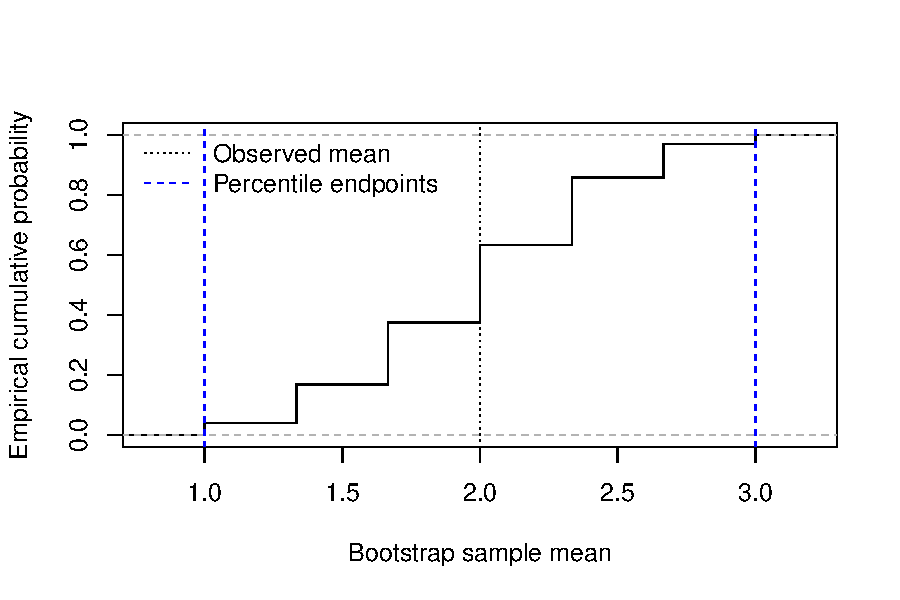
\includegraphics[width=\linewidth]{figures/bootstrap/bootstrap-distribution-1} 

}


\end{knitrout}

\caption[Empirical cumulative distribution of bootstrap means]{
Empirical cumulative distribution of 2,000 bootstrap means from the
observations 1, 2, and 3, using seed 20260927. The dotted line marks the
observed mean of 2; dashed lines mark the 95 percent percentile interval
endpoints of 1 and 3. This small-sample example illustrates computation,
not reliable coverage.}
\label{fig:bootstrap-distribution}
\end{figure}

Figure~\ref{fig:bootstrap-distribution} is generated by the R chunk.
Its caption and label are set explicitly with LaTeX commands in this Rnw
source. Use \verb|\ref| to refer to the figure number in the text.
The shorter caption appears in the list of figures; the full caption
explains the data and line styles.


\paragraph{Software versions.}
The following output records the versions used to generate this appendix.

\begin{knitrout}
\definecolor{shadecolor}{rgb}{0.969, 0.969, 0.969}\color{fgcolor}\begin{kframe}
\begin{verbatim}
## R version 4.6.1 (2026-06-24) 
## knitr 1.51
\end{verbatim}
\end{kframe}
\end{knitrout}



For a research application, accompany computational output with an
interpretation of what it establishes and which assumptions it requires.
Report relevant software versions and simulation settings, and use informative
captions and numbered cross-references to connect figures with the discussion.
Follow \citet{schifano2026statistical} for further guidance on statistical
writing and the presentation of tables and figures.


\singlespacing
\bibliographystyle{apalike}
\bibliography{thesis}
\end{document}
